\chapter{The Asynchronous Model and the FLP Impossibility Theorem (1)}
\section{Relaxing the Synchronous Assumption}
The chapters 4 and 5 introduce the asynchronous model of communication and prove what is possibly the most famous impossibility result in distributed computing, the FLP impossibility
theorem. This will probably be the longest and trickiest proof that we do in the entire chapter
series. Understanding it will be a feather in your cap and put you in quite rarified company.


\subsection{Recap and Context}
Chapter 2 presented the Dolev-Strong protocol as a solution to the Byzantine broadcast
problem. That protocol satisfied termination, agreement, and validity, no matter how many
nodes were Byzantine (i.e., could deviate arbitrarily from the protocol). Using the DolevStrong protocol as a subroutine,
we constructed an equally fault-tolerant protocol for the (multi-shot) state machine replication (SMR) problem satisfying consistency and liveness.
We proved these guarantees for the Dolev-Strong protocol (and hence our SMR protocol)
under three assumptions. First, that the set of nodes and their names are known a priori
(the “permissioned setting”). We will continue to make this assumption in these chapters
(waiting until chapter 9 to relax it, in the context of sybil-resistance and proof-of-work).
Second, the “public key infrastructure (PKI)” assumption, secure digital signature schemes
exist, every node has a distinct public key-private key pair, and all nodes’ public keys are
common knowledge at the start of the protocol. As we saw in Chapter 3, the PKI assumption
fundamentally changes whether or not the Byzantine broadcast problem is solvable in the
synchronous model (with $f \geq \frac{n}{3}$, where $n$ is the number of nodes and $f$ is the maximum
number of Byzantine nodes). In the asynchronous model studied in these lessons, it turns
out not to matter (the FLP impossibility theorem holds even with the PKI assumption).
The third assumption is  that at least some
of the nodes run the protocol honestly.
By honest that means without any
intentional or unintentional deviation
from what the protocol prescribes and
we'll use a parameter $f$ to denote
an upper bound on how many nodes cannot
be honest and how many nodes might deviate from what the protocol prescribes. In a blockchain setting,
the most appropriate model for a
node which is not honest is to assume
it's controlled by an attacker. So we call it
something known as a byzantine node. We
basically make no assumptions about the
behavior of byzantine nodes. We might
assume something like they can't break
cryptography but they can try to
manipulate the protocol in any way that they like.
The fourth assumption (really, two subassumptions) is the one we’re keen to relax in this
chapter: (i) all nodes share a global clock (common notion of time); (ii) every message sent during a time step $t$ arrives
at its destination prior to the start of time step $t + 1$. We might be able to live with (i),
but (ii) is completely unreasonable for a protocol operating over the Internet. For example,
if we define time steps (rather generously) to be two seconds long, then under “normal
operating conditions” we might expect subassumption (ii) to hold. But we all have firsthand experience with Internet delays longer than two seconds. 
There are a million reasons why this could happen. Maybe the Internet (or at least your neighborhood in it) is congested,
with lots of packets getting dropped and retransmitted. Maybe the BGP routing protocol is
having a really bad day and sending packets along highly suboptimal routes. Maybe there
are some serious network outages. Or maybe the delays are being caused deliberately by a
malicious actor— a “denial-of-service (DoS)” attack.

\subsection{Time Inflation: Failed Attempts at Relaxing the Model}
Maybe the simplest way to relax the problematic subassumption (ii) in the synchronous
model is to allow a message to be delayed up to some number of time steps—for example,
perhaps every message arrives after somewhere between 1 and 100 time steps. Unfortunately,
this idea does not really generalize the synchronous model at all. Think about the DolevStrong protocol, for instance. In that protocol, the sender sent out messages at time step 0, and the non-senders exchanged cross-checking messages in time step 1, time step 2, and so
on. If we’re told that messages might get delayed up to 100 time steps, the obvious response
is to have the non-senders instead exchange messages only at time step 100, time step 200, and so on. The behavior and guarantees of the modified protocol then match those of the original protocol in the original model.\\
This attempt at relaxing the synchronous model is deeply unsatisfying for two semi-related reasons. First, it did not force us to confront the main issue, that a protocol operating over the Internet necessarily must deal with unexpected outages and attacks. Second, it
naturally led us to stupid protocols that spend most of their time idle. For example, in the
time-inflated version of the Dolev-Strong protocol, even if all the sender’s messages arrive
at the non-senders by time step 1, the non-senders will wait until time step 100 before
doing anything, just to make sure that everybody has the chance to receive all the messages
destined to them.\\
A practical protocol can’t afford to have its speed dictated by the worst-possible message
delay, and should be fast whenever the underlying communication network is fast. This is
the basic intuition behind (one version of) the partially synchronous model, discussed in
chapter 6. But first, let’s explore what’s possible with only the most minimal assumptions
about the reliability of message delivery.

\section{The Asynchronous Model}
\noindent
\textbf{Informal description.} The asynchronous model of communication represents the polar opposite of the synchronous model, with the two subassumptions replaced by nonassumptions. First, there will be no shared global clock, and thus no (even approximately)
shared notion of time. Second, messages may suffer arbitrarily long (finite) delays—a protocol designed for the asynchronous model must be ready for anything.
The asynchronous model does make a minimal assumption about message delivery. Every
message is eventually delivered to the intended recipient. (Without this assumption, it’s
possible that no messages ever arrive and trivially consensus is impossible to reach. We
want to show that consensus is impossible even if all messages eventually arrive.) There is
no priori bound on how long delivery takes for any given message, however—it may 
arrive after the delivery of one billion other messages that were sent after it.\\

\noindent
\textbf{Formal description.} To rigorously prove an impossibility result, we need a completely
formal mathematical model. Here it is:
\nt{
\begin{center}
    \textbf{The Asynchronous Model}
\end{center}
\begin{itemize}
    \item $M$ denotes the pool of outstanding (not-yet-delivered) messages (initialized to $\{(r, \bot)\}^n_{r=1}$)
    The model is completely event driven and there's no notion of time. Messages are only going to be sent in response of messages that are received.
    \item while(TRUE):
    \begin{itemize}
        \item an arbitrary message $(r, m) \in M$ is delivered to recipient $r$ while $m$ is the message content. (subject to the eventual delivery constraint)
        \item $r$ can add any number of messages to $M$. In this model, we make no assumptions about message delays and in particular there's no promises about the ordering. For example, if one message was sent prior to another, there's no guarantee that it's going to be received prior to another.
    \end{itemize}
\end{itemize}
}

It might be helpful to think of the iterations of the main while loop as time steps, but keep
in mind that, in the asynchronous model, nodes have no idea how many iterations have
been executed. A message $(r, m)$ sent by a node specifies two things, the recipient $r$ (one of
the $n$ nodes) and the payload m (which is arbitrary content). The model is purely event-driven, with messages sent by a node only in response to receiving a new message. Every sent message $(r, m)$ will be delivered eventually (to $r$), but the order in which messages
are delivered is arbitrary. Given that our goal is to design a consensus protocol that has
provable guarantees, no matter what the order of message deliveries, it’s useful to think of
each iteration’s message as being chosen by an “adversary” whose sole goal is to fail the
consensus protocol.\\

\noindent
\textbf{Ensuring participation through dummy messages.} If the message pool $M$ starts out
empty, no messages ever get delivered and hence no messages ever get sent. So to get the
ball rolling, let’s initialize the message pool $M$ with one dummy message $(r, \bot)$ for each
node $r$—because all these messages must eventually be delivered, all nodes will eventually
get the chance to participate. You might respond that nodes should be able to participate
many times, not just once. This is easily ensured with a convention for what protocols do—
let’s assume that, whenever a node $r$ receives a message $(r, m)$, it either terminates or sends
a dummy message $(r, \bot)$ to the pool $M$ (along with possibly many other messages). This
way, every node can participate in the protocol for as long as it wants.\\
Another assumption that we make is that all messages are eventually delivered. It could be an arbitrarily large but finite amount of time. This is sort of a minimal assumption for the model to be interesting. Otherwise, for instance a bunch of honest nodes could just be starved till the end of time and in this case, obviously we cannot maintain consistency and liveness.

\noindent
\textbf{A conspiracy of adversaries.} In Chapters 2 and 3 we learned first-hand the challenges of
consensus protocol design in the presence of multiple Byzantine nodes—because Byzantine
nodes can do literally anything (other than break cryptography), they might deviate
from the intended protocol in a coordinated way, conspiring to fail its design goals.
In the asynchronous model, a conspiracy among Byzantine nodes picks up a new, powerful
ally—adversarial message delivery. For a protocol to be robust to both Byzantine nodes
and adversarial message delivery, it must in particular survive conspiracies between them.
 Perhaps with message delays enabling the shenanigans of the Byzantine nodes. In effect, the
actions of all the Byzantine nodes and the choices of which messages to deliver, are controlled
by a single malicious actor. The power of this actor is what makes protocol design in the
asynchronous model so challenging.\\

\noindent
\textbf{Interpreting the asynchronous model.} Your response to the asynchronous model might
be that it doesn't seem very realistic—who is this all-powerful actor who can dictate which
messages are received when in the Internet? And that’s true. But the point of the asynchronous model 
is absolutely not to faithfully model communication over the Internet.
Rather, the point is to avoid making any assumptions about how that communication works.
Remember in Chapter 2, when we talked about how the interpretation of Byzantine nodes
has evolved with technology over the decades? Back in the 1980s and 1990s (e.g., with IBM
replicating a database for higher uptime), researchers in distributed computing thought hard
about protocols resilient to Byzantine nodes. They did this not because they were literally
worried about malicious actors, but rather because they wanted to avoid any (necessarily
limited and controversial) assumptions about how a node with buggy software might behave.
Fast forward to the present and the context of blockchains securing billions of dollars, and
we very much do want to literally model malicious actors whose sole goal is screw up our
protocol.\\
The asynchronous model makes no assumptions about message delivery for the same
reasons researchers in the 1980s often made no assumptions about the behavior of faulty
nodes—the alternative of imposing specific and hard-to-justify constraints would be much
worse.\\
It’s dangerous to put much stock in a protocol whose guarantees are predicated on an
overly specific model of “communication over the Internet.” Even if that model is valid now,
why should it be valid tomorrow? So, if you're designing a consensus protocol, this would be the dream because we like to have a consensus protocol that has nice qualities even under these completely minimal assumptions. The dream, then, is to design a consensus protocol that
works in the asynchronous model, in the absence of any assumptions (other than eventual
message delivery). Such a protocol would automatically be interesting, because it would
give you the functionality you want even with a barely functioning communication network.
Alas, as we’ll see, this dream cannot be realized without pulling back some from the extreme
lack of assumptions of the asynchronous model.


\section{Byzantine Agreement}
The FLP impossibility theorem concerns a (famous) consensus problem that we’ve not yet
discussed, Byzantine agreement. Before defining it, let’s be clear on what we mean by a
“protocol.”\\

\noindent
\textbf{Protocols.} As usual, a protocol is a piece of code deployed locally at each node that specifies what
the node should do—that is, what messages it should send—as a function of what the
node knows. Keep in mind that the asynchronous model is purely event-driven, and so the
protocol is invoked at a node upon receipt of a new message. At that moment in time, the node knows exactly two things: (i) whatever private input it started the protocol with; (ii) whatever sequence of messages it has received thus far. A protocol therefore specifies, for
every possible value of (i) and (ii), the messages that a node should send in response to the
most recently received message. We stress that the prescription made by a protocol cannot
depend on information that a node does not know (e.g., the message sequences that have
been received by other nodes). If two different  runs of a protocol result in the exact same
sequence of messages getting delivered to a node (and the private input is the same in both
runs), then that node will behave identically in the two runs (and in particular will output
the same thing either way).\\

\noindent
\textbf{The Byzantine agreement problem.} The Byzantine agreement (BA) problem is a
single-shot consensus problem, similar to the Byzantine broadcast (BB) problem studied
in Chapters 2 and 3. Unlike the BB problem, in the BA problem there is no distinguished
sender node—all the nodes play the same role. In the BB problem, the sender is the only
node with a private input. In the BA problem, every node $i$ has a private input $v_i$, drawn
from some known set $V$ of possible values. (In a blockchain context, $v_i$ might be an ordering of the as-yet-unexecuted transactions that $i$ knows about and $V$ the set of all possible such sequences. For this chapter’s impossibility result, we’ll only need to consider the case
with $V = \{0, 1\}$.) As usual, “private” means that, when the protocol commences, nobody
other than node i knows anything about what $v_i$ is (other than that it is some element of $V$).\\

\noindent
\textbf{Desired protocol properties.} What constitutes a “solution” to the Byzantine agreement
problem? Like Byzantine broadcast, we’re interested in protocols that satisfy three properties: termination, agreement (the safety property), and validity (the liveness property). Termination and agreement are defined exactly as in the Byzantine broadcast problem. The
validity property needs to be modified to reflect the fact that all nodes have a private input
rather than just one. Intuitively, if all the honest nodes begin the protocol with no disagreement among their private inputs, then their outputs should match their inputs (i.e., Byzantine nodes should not be able to trick them into deviating from their common input).
Formally:
\nt{
\begin{center}
    \textbf{Desired Properties of a Byzantine Agreement Protocol}
\end{center}

\begin{enumerate}
    \item \textbf{Termination.} Every honest node $i$ eventually halts with some output $w_i \in V$.
    \item \textbf{Agreement.} All honest nodes halt with the same output (no matter what the private inputs are).
    \item \textbf{Validity.} If $v_i = v^*$ for every honest node $i$, then $w_i = v^*$ for every honest node $i$.
\end{enumerate}
}
As usual, what’s hard is getting all the properties simultaneously. Termination and agreement by themselves are trivially achievable (with all honest nodes always outputting a default value $\bot$), and similarly for termination and validity (with honest nodes outputting their private inputs).\\

\noindent
\textbf{Why a third consensus problem?} You might be annoyed that we’ve introduced yet
another consensus problem. Why not prove an impossibility result directly for the BB or
SMR problems? (The BA problem is actually the most canonical of the three, but that’s
not the main reason.)\\
In the asynchronous model, Byzantine broadcast turns out to be trivially unsolvable.
Meanwhile, the BA problem captures the essence of why consensus is impossible in the
asynchronous model. In particular, the FLP impossibility result for the BA problem implies
the impossibility of SMR in the asynchronous model, which is arguably the result that we
really care about.

\section{The FLP Impossibility Theorem}
Now that we understand the asynchronous model, what we mean by a protocol in this
model, and the definition of the Byzantine agreement problem, we’re in a position to state
the famous FLP impossibility theorem (here “FLP” stands for the three researchers who
proved it: Fischer, Lynch, and Paterson). The theorem states that, even with only a single
Byzantine node, there is no deterministic protocol that solves the Byzantine agreement
problem in the asynchronous model.\\

\thm{FLP Impossibility Theorem [2]}{For every $n \geq 2$, even with $f = 1$, no
deterministic protocol for the Byzantine agreement problem satisfies termination, agreement,
and validity in the asynchronous model.}

Several comments:\\
\begin{itemize}
    \item Here “deterministic” means that nodes do not locally flip any random coins—the messages sent out by a node in response to a newly received message are completely
    determined by its private input and the messages it has received thus far.
    \item The FLP impossibility theorem also has implications for randomized protocols (in
    which the messages sent out by a node can be a probabilistic function of their private
    input and received messages). What its proof really shows is that, for every protocol
    (deterministic or randomized) that is guaranteed to satisfy agreement and validity upon
    termination, there exists a non-terminating run of the protocol (while still satisfying
    the eventual delivery property). Thus, no randomized protocol can guarantee all three of the properties that we want all of the time. The best we can hope for from a
    randomized protocol that guarantees agreement and validity upon termination are
    probabilistic guarantees on termination (e.g., a small expected running time, a bounded
    running time with high probability, and/or a finite running time with probability 1).
    \item Guaranteeing consensus gets harder as $f$, the maximum number of Byzantine nodes,
    grows larger. Thus the most impressive possibility results are the ones with large values
    of $f$ (the Dolev-Strong protocol being an extreme example). For the same reason, the
    most impressive impossibility results are the ones that hold even with small values
    of $f$. The fact that the FLP impossibility theorem holds even with $f = 1$ is in this
    sense the strongest result possible!
    \item The statement of Theorem 4.4.1 above actually undersells the FLP impossibility theorem,
    which holds even with a single crash fault. (As discussed in Chapter 2, a crash fault
    is the special case of a Byzantine node that follows the protocol honestly up to some
    moment in time at which someone pulls the node’s plug. After that point, the node
    neither receives nor sends any further messages for the rest of the protocol’s run. Such
    a node cannot, for example, deliberately send out conflicting messages to different
    nodes.) We’ll prove the theorem assuming one Byzantine node. A good exercise for you
    is to extend the proof (via a couple of minor tweaks) to hold more generally with one
    crash fault. To think about it, there's no solution to Byzantine Agreement problem without a solution for the Byzantine Broadcast either because from the latter we can build the former.
    \item The impossibility result continues to hold under the PKI assumption. (If you think about it, this is an automatic consequence of the previous point.)
    \item Theorem 4.4.1 formally separates what is possible in the synchronous and asynchronous
    models and shows that, as intuition might suggest, consensus is fundamentally more
    difficult in the latter model.
    \item Don’t forget! the point of an impossibility result is not to discourage anybody from
    trying to come up with practical solutions to a problem. It’s to properly educate
    everybody about the compromises required. (as exemplified by the partially synchronous
    model in Chapter 6)
\end{itemize}

The question is why is the FLP impossibility theorem true?

\section{Proof of Theorem 4.4.1: Configurations}
Like the PSL-FLM impossibility result in chapter 3 (for Byzantine broadcast in the synchronous model with $f \geq \frac{n}{3}$ and without the PKI assumption), we’ll proceed by contradiction. That is, we’ll assume that there is in fact a deterministic protocol $\pi$ for the Byzantine
agreement problem that is guaranteed to satisfy termination, agreement, and validity in
the asynchronous model with $f = 1$. Deriving a contradiction from this assumption would
show that $\pi$ can’t exist. The specific plan is to show that, by virtue of $\pi$ satisfying agreement and validity upon termination, there will inevitably be cases in which it runs forever(contradicting termination).\\

\noindent
\textbf{Protocol runs as walks in a directed graph.} Given a protocol $\pi$, we need to exhibit
an infinite sequence of things that can happen without the protocol terminating. To make
sense of this, let’s define a configuration as a snapshot of a protocol’s trajectory—information
sufficient to restart the protocol from where it left off. Precisely, a configuration includes:
\begin{itemize}
    \item the current state of the message pool $M$
    \item the private input of each of the nodes
    \item the sequence of messages received thus far by each of the nodes
\end{itemize}

You can think of a protocol’s run as a walk through a big (possibly infinite) directed graph,
with vertices corresponding to configurations $C$ and edges corresponding to message deliveries $C \xrightarrow[]{(r,m)} C'$ (Figure 4.1). Note that whenever a message $(r, m) \in M$ is delivered, the configuration changes in three ways: 
\begin{enumerate}[label=(\roman*)]
    \item $(r, m)$ is removed from the pool $M$
    \item the delivered message is appended to the end of r’s sequence of messages received thus far
    \item newly sent messages (by $r$, as prescribed by $\pi$ or by $r$’s Byzantine strategy) are inserted
into $M$. Exhibiting a sequence of message deliveries for which $\pi$ runs forever (contradicting
termination) is tantamount to exhibiting an infinite path in this directed graph.
\end{enumerate}\\

\noindent
\textbf{Three types of configurations.} The next definition classifies configurations into three
categories. Assume that the private input of every node is either 0 or 1 (i.e., $V = \{0, 1\}$).\\

\begin{figure}[h]
    \centering
    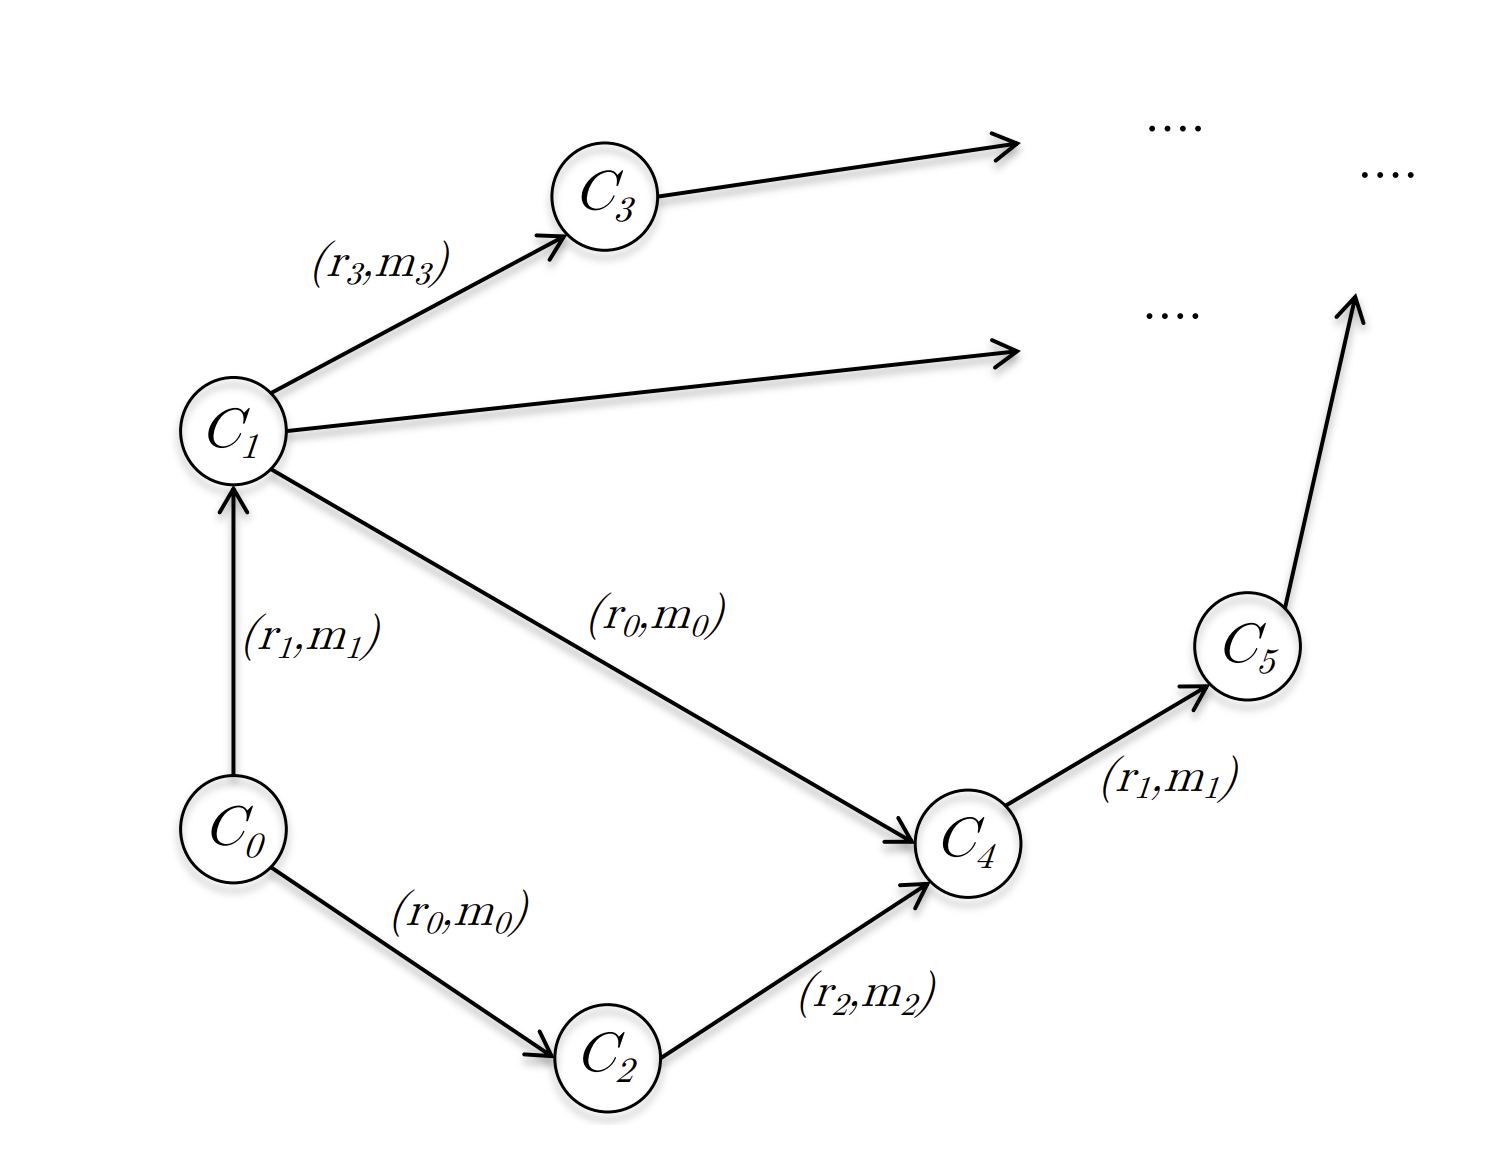
\includegraphics[scale = 0.5]{figures/f14.png}
    \caption{A run of a protocol can be visualized as a walk through a directed graph, with
    vertices corresponding to configurations and edges to message deliveries.}
    \label{fig:mesh1}
\end{figure}\\

Because $\pi$ satisfies agreement (by assumption), whenever $\pi$ terminates, there are only two
possible outcomes: either all the honest nodes output 0 (the “all-zero outcome”), or they all
output 1 (the “all-one outcome”).
\dfn{0-, 1-, and Ambiguous Configurations}{A configuration is:\\
\begin{itemize}
    \item[--] a 0-configuration if all possible strategies of the Byzantine nodes and all possible sequences of message deliveries lead to the all-zero outcome;
    \item[--] a 1-configuration if all possible strategies of the Byzantine nodes and all possible sequences of message deliveries lead to the all-one outcome;
    \item[--] an ambiguous configuration if it is neither a 0-configuration nor a 1-configuration.
\end{itemize}}

Because $\pi$ satisfies termination and agreement, we can equivalently define an ambiguous
configuration as one from which there exist strategies for the Byzantine nodes and a sequence
of message deliveries that lead to the all-zero outcome, and also such strategies and such
a sequence that lead to the all-one outcome. From a 0- or 1-configuration, the eventual
outcome is a foregone conclusion. (no matter what the conspiracy of adversaries does) From an
ambiguous configuration, the adversary can force whichever outcome it prefers. Definition 6.1
is with respect to a fixed protocol $\pi$. For example, a given configuration may be ambiguous
with respect to one protocol but not ambiguous with respect to another.\\

\noindent
\textbf{High-level proof plan.} The proof will hunt for an infinite path in the directed graph in
Figure 4.1, and specifically for an infinite sequence of ambiguous configurations (with respect
to the assumed correct protocol $\pi$). This will contradict the assumption that $\pi$ satisfies
termination and complete the proof.\\
To exhibit such a sequence, we’ll use two lemmas, the first playing the role of a base
case and the second of an inductive step in a proof by induction. Lemma 4.6.1 will get us
started—it states that there exists a choice of nodes’ private inputs so that the corresponding
initial configuration $C_0$ is ambiguous. Lemma 5.1.1 will then show how to exhibit a new
ambiguous configuration $C_{i+1}$ from an old one $C_i$. Applying Lemma 4.6.1 once and then
Lemma 5.1.1 over and over again produces an infinite sequence $C_0 \to C_1 \to C_2 \to C_3 \to \cdots$
of ambiguous configurations, which is exactly what we wanted. Neither of these lemmas is
obvious. Lemma 4.6.1 is a bit easier to prove (and it doesn't rely on the full power of the
adversary in the asynchronous model), so let’s start with that one.

\section{Proof of Theorem 4.4.1: Initial Ambiguity}
Here’s the formal statement of the lemma that will kick off an infinite sequence of ambiguous
configurations.\\
\mlemma{An Initial Ambiguous Configuration}{For every deterministic protocol $\pi$
that satisfies agreement and validity upon termination (with $f = 1$ and some $n \geq 2$), there
exists a choice of nodes’ private inputs such that the corresponding initial configuration is
ambiguous.}
Configurations in general can get pretty crazy (e.g., with billions of messages in the
message pool), but there are only $2^n$ possible initial configurations: at the start of the
protocol, the message pool $M = \{(r, \bot)\}^n_{r=1}$ is uniquely determined and all nodes have
received an empty sequence of messages, so the only degree of freedom is the choice of
nodes’ private inputs (and with n nodes and all private inputs 0 or 1, there are $2^n$
such choices). In fact, we’ll only need to consider n − 1 of the $2^n$
initial configurations to identify
an ambiguous one.\\

\begin{myproof}
Visualize nodes’ private inputs as an n-bit string, with the $i$th bit
indicating node $i$’s private input. Imagine starting from the all-0s string and flipping 0s to 1s
one-by-one from left-to-right, ending in the all-1s string. This process generates a total of $n+1$
choices for the private inputs, with corresponding initial configurations $X_0, X_1, X_2, \cdots, X_n$(Figure 4.2). (In $X_i$
, the first $i$ nodes have a private input of $1$ and the last n − i nodes have a private input of 0.)\end{myproof}\\

Next let’s invoke the assumption that $\pi$ satisfies validity. Validity implies that when
all nodes’ inputs are 0 (and in particular those of the honest nodes are 0), as they are in
the configuration $X_0$, the protocol must terminate in the all-zero outcome (no matter the
strategy of Byzantine nodes and the sequence of message deliveries). In the terminology of Definition 4.5.1, the initial configuration $X_0$ must be a 0-configuration. Invoking validity again, by the same argument, the initial configuration $X_n$ (in which all nodes’ inputs are 1) must be a 1-configuration.

\begin{figure}[h]
    \centering
    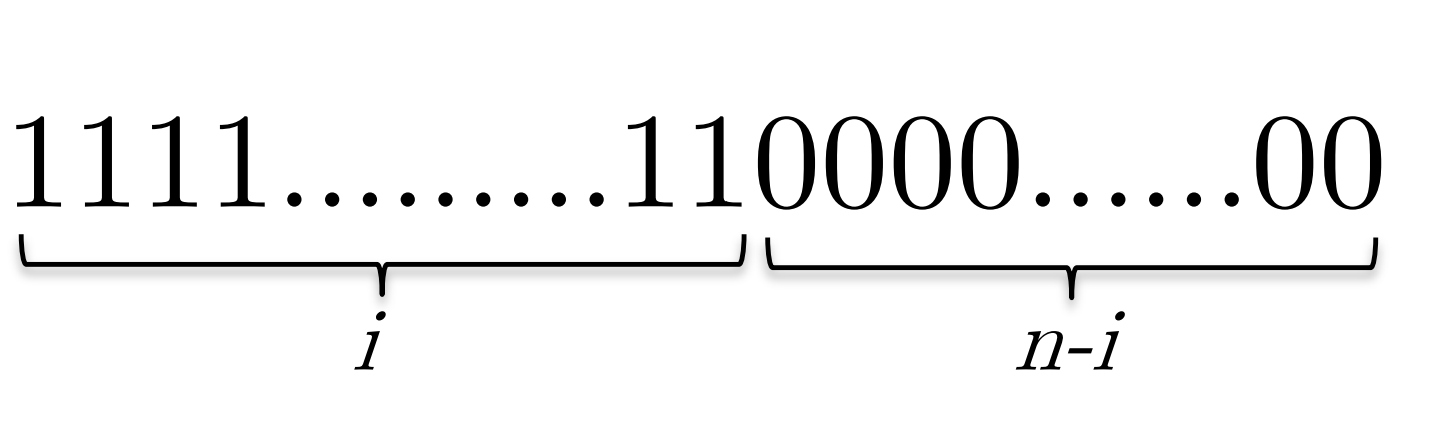
\includegraphics[scale = 0.5]{figures/f15.png}
    \caption{ In the initial configuration $X_i$, nodes $1, 2, \cdots, i$ have a private input of 1 and nodes $i + 1, i + 2, \cdots, n$ have a private input of 0.}
    \label{fig:mesh1}
\end{figure}\\

We claim that one of the intermediate configurations $X_1, X_2, \cdots, X_{n−1}$ must be an ambiguous configuration (in which case, we’ll be done with the proof). To see this, consider the smallest value of $i \geq 1$ such that $X_i$
is not a 0-configuration. (This value must exist because,
if nothing else, the choice $i = n$ would meet the criterion.) By the choice of $i$, $X_{i−1}$ must be
a 0-configuration (otherwise, we could have taken i to be smaller).
If $X_i$ is an ambiguous configuration, we’re done. The only worry is that $X_i$ might be
a 1-configuration—i.e., that flipping the private input of node $i$ from 0 to 1 jumps directly
from a 0-configuration to a 1-configuration. Intuitively, such a “pivotal” private input should
sound implausible—if node $i$ happens to be Byzantine, it is fully capable of hiding its private
input from the rest of the nodes and keeping them in the dark. To make that idea precise,
suppose node $i$ is Byzantine and consider two possible strategies for it:\\
\begin{enumerate}
    \item any strategy that forces the all-one outcome (which must exist, given that $X_i$ is not a 0-configuration);
    \item the strategy in which it pretends its private input is actually 0 and otherwise it follows the protocol $\pi$ honestly.
\end{enumerate}
With strategy (2), the trajectory of the protocol $\pi$ is exactly the same as its trajectory from
the initial configuration $X_{i−1}$ when all nodes follow $\pi$ honestly. (All honest nodes see the
exact same sequences of messages either way, and hence operate identically in both cases.)
Because $X_{i−1}$ is a 0-configuration (by our choice of $i$), the protocol must terminate in the
all-zero outcome. We conclude that the Byzantine node $i$ has the option of forcing either the
all-zero or the all-one outcome from $X_i$, and thus $X_i$ is indeed the ambiguous configuration that we’re looking for.

\begingroup
\let\clearpage\relax
\begin{thebibliography}{5}
\bibitem{texbook}
S. Duan, M. K. Reiter, and H. Zhang. BEAT: Asynchronous BFT made practical. In \textit{Proceedings of the ACM SIGSAC Conference on Computer and Communications Security},
pages 31–42, 2018. URL: https://www.csee.umbc.edu/~hbzhang/files/beat.pdf.

\bibitem{lamport94}
M. J. Fischer, N. A. Lynch, and M. S. Paterson. Impossibility of distributed consensus
with one faulty process. \textit{Journal of the ACM}, 32(2):374–382, 1985. URL: https://
groups.csail.mit.edu/tds/papers/Lynch/jacm85.pdf.

\end{thebibliography}
\endgroup

\newpage
\chapter{The Asynchronous Model and the FLP Impossibility Theorem (2)}
\section{Proof of Theorem 4.4.1: Reduction to Lemmas 4.6.1 and 5.1.1}
Let’s move on to the notorious second lemma, which is fairly similar to the first one but
definitely a bit trickier. This lemma acts like an inductive step in a proof by induction, that it takes as input a sequence of ambiguous configuration and outputs a longer such sequence. The two lemmas can then be used to exhibit the desired infinite sequence of
ambiguous configurations: Lemma 4.6.1 gets the sequence started, and applying Lemma 5.1.1 over and over again produces the rest of it.\\

\noindent
\textbf{Statement of the second lemma.} Actually, the argument above misses a subtle point.
That subtle point is the reason that the statement of the second lemma is perhaps more complex
than you were expecting (Figure 5.1):

\mlemma{Extending an Ambiguous Sequence}{Fix a deterministic protocol $\pi$ that
satisfies agreement and validity upon termination (with $f = 1$ and some $n \geq 2$). Let $C_i$
denote an ambiguous configuration and $(r, m)$ a message in $C_i$’s message pool. Then, there
exists a sequence of message deliveries such that:\\
\begin{enumerate}
    \item the last step of the sequence is the delivery of $(r, m)$
    \item the end of the sequence is an ambiguous configuration $C_{i+1}$
\end{enumerate}}

Another way of saying this is Lemma 5.1.1 guarantees that
there is a way to eventually deliver the
message in question $(r,m)$
while remaining in an ambiguous configuration. 
\begin{figure}[h]
    \centering
    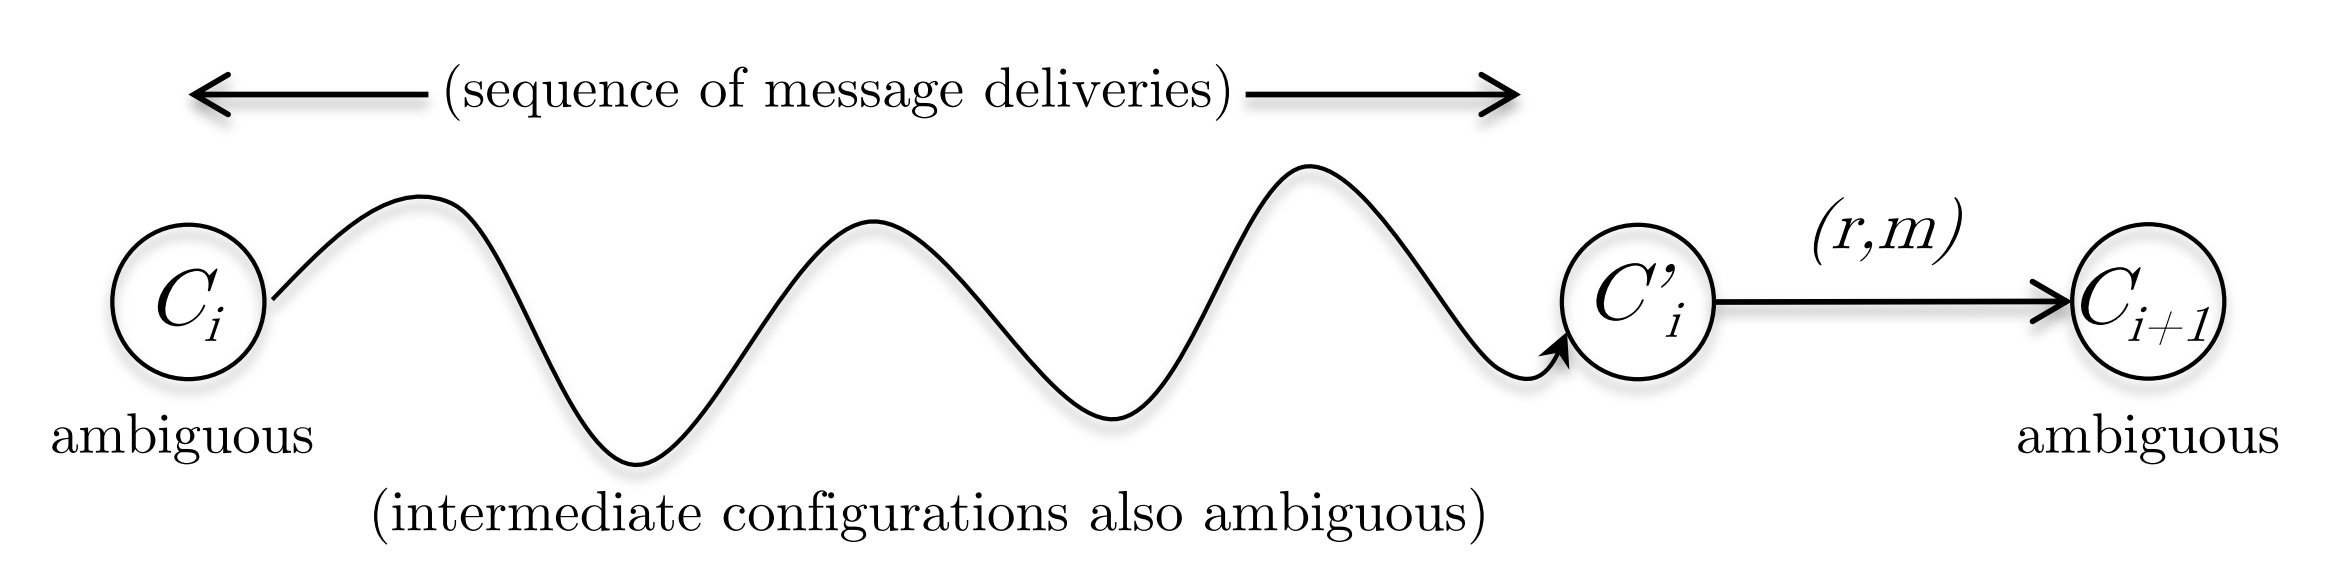
\includegraphics[scale = 0.5]{figures/f16.png}
    \caption{ Lemma 5.1.1: extending a sequence of ambiguous configurations (from $C_i$ to $C_{i+1}$) while delivering the message $(r, m)$ last.}
    \label{fig:mesh1}
\end{figure}\\

You might have been expecting a simpler statement: for every ambiguous configuration $C_i$, there exists a message to deliver, resulting in another ambiguous configuration $C_{i+1}$. What’s up with forcing the lemma to work with arbitrarily chosen message $(r, m)$ that’s hanging out in $C_i$’s message pool?\\
The simpler statement is trivially true: start from the initial ambiguous configuration $C_0$
promised by Lemma 4.6.1 and then deliver an infinite sequence of dummy messages (messages of the form $(r, \bot)$, see Section 4.2). The dummy messages don’t do anything, so all of the configurations produced will be ambiguous. Unfortunately, iterated application of this
simpler statement yields a sequence in which the adversary never delivers any (non-trivial)
messages. Of course consensus is impossible if we allow an adversary to do this! This issue
is exactly why, in the definition of the asynchronous model in Section 4.2, we insisted on the constraint that every message sent to the message pool must eventually be delivered to its intended recipient.\\

The extra complexity in the statement of Lemma 5.1.1 addresses this exact issue, allowing
us to produce an infinite sequence of configurations that satisfies the eventual delivery constraint. Formally, here’s the proof that Lemma 4.6.1 and (the as-yet-unproven) Lemma 5.1.1 in tandem imply the FLP impossibility theorem:\\
\noindent
\textit{Proof of Theorem 4.4.1:} Fix a deterministic protocol $\pi$ that satisfies agreement and validity
upon termination (with $f = 1$ and some $n \geq 2$). No prizes for guessing the first step: invoke
Lemma 4.6.1 to choose an initial configuration $C_0$ that is ambiguous (which must exist).\\
Presumably we then want to invoke Lemma 5.1.1 over and over. Each invocation asks
us to pick a message $(r, m)$ in the current message pool—how should we choose? Putting
Lemma 5.1.1 aside for a moment, imagine we didn't care about retaining ambiguity and
just wanted to make sure that every message eventually gets delivered. An easy solution
would be first-in first-out (FIFO), meaning that always deliver the message in the message pool that was
sent the largest number of iterations ago (even if it forces a transition from an ambiguous
configuration to a 0- or 1-configuration). Then, whenever a message is added to the existing
message pool $M$, we know that it will be delivered $|M|$ iterations later (here $|M|$ denotes
the number of messages in the pool). Because $M$ is always finite (we only allow a node to
add a finite number of messages in a single iteration), every message gets delivered after a
finite number of iterations.\\
Lemma 5.1.1 is phrased so that we can split the difference between the trivial solution
that guarantees never-ending ambiguity but not eventual delivery (i.e., deliver only dummy
messages) and the FIFO solution that guarantees the latter but not the former. The key idea
is to simulate FIFO message delivery as closely as possible subject to retaining ambiguity.
Precisely, here’s how we’ll define our sequence of ambiguous configurations:
\begin{itemize}
    \item define $C_0$ as the ambiguous configuration promised by Lemma 4.6.1;
    \item for $i = 0, 1, 2, \cdots$:
    \begin{itemize}
        \item let $(r_i, m_i)$ denote the oldest message in $C_i$’s message pool,
        \item define $C_{i+1}$ as the ambiguous configuration promised by Lemma 5.1.1 (with respect to $C_i$ and $(r_i, m_i)$).
    \end{itemize}
\end{itemize}

This procedure constructs a sequence of sequences—there could be a billion intermediate
configurations between some $C_i$ and $C_{i+1}$ (Figure 5.2)—but whatever, the concatenation of
these sequences is itself a sequence of configurations. The sequence between $C_i$ and $C_{i+1}$ is
effectively stalling (delivering whatever messages it wants, preserving ambiguity) up to the
point at which it can deliver the message $(r_i, m_i)$ without resolving the ambiguity.\\
By Lemma 4.6.1 and 5.1.1, all of the $C_i$’s—and hence, also all of the intermediate configurations—are ambiguous configurations. The eventual delivery constraint is satisfied by this sequence for the same reason that FIFO delivery satisfies it: if a message $(r, m)$ gets added to a message pool M at or before a configuration $C_i$, it is guaranteed to be delivered by configuration $C_{i+|M|}$ at the latest. (Each invocation of Lemma 5.1.1 will
deliver at least one of the $|M|$ messages that preceded $(r, m)$. After at most $|M|$ invocations,
$(r, m)$ will be first in line.)\\
\begin{figure}[h]
    \centering
    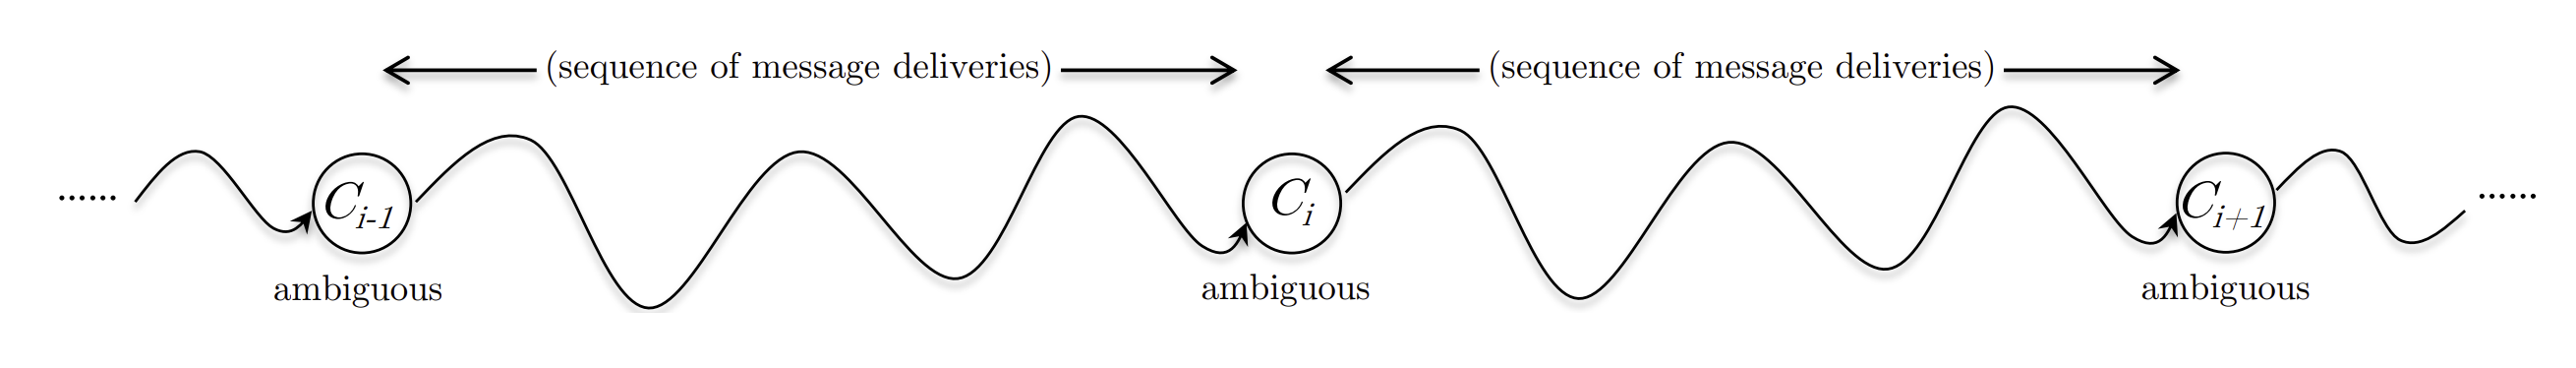
\includegraphics[scale = 0.5]{figures/f17.png}
    \caption{Repeated applications of Lemma 5.1.1 produces an arbitrarily long sequence (equivalently, sequence of sequences) of ambiguous configurations.}
    \label{fig:mesh1}
\end{figure}\\
Now we know that Lemma 4.6.1 is true and that Lemmas 4.6.1 and 5.1.1 imply the FLP impossibility result. The final order of business is to prove Lemma 5.1.1.
\newpage
\section{Proof of Theorem 4.4.1: Extending an Ambiguous Sequence}
To prove Lemma 5.1.1, fix a deterministic protocol $\pi$ that satisfies agreement and validity
upon termination (with $f = 1$ and some $n \geq 2$), an configuration $C_i$, and a message $(r, m)$
belong to $C_i$’s message pool. We need to show that it’s possible to eventually deliver $(r, m)$
while retaining ambiguity (possibly delivering a billion other messages in the meantime).

\subsection{Proof Setup}
Next we classify configurations into three categories. Like the classification in Section 4.5, this
one will be defined with respect to the fixed protocol $\pi$. Unlike the one in Section 4.5, it will
also be defined with respect to the fixed configuration $C_i$ and message $(r, m)$.
If delivering the message $(r, m)$ at the configuration $C_i$ happens to lead directly to another
ambiguous configuration, then we’re done and there’s nothing more to prove. So suppose
delivering $(r, m)$ immediately would lead to a 0-configuration, with the eventual outcome
forced to be the all-zero outcome. (The argument for the case in which it leads to a 1-
configuration is exactly the same, reversing the roles of 0 and 1.)\\
Here are the additional three categories of configurations that we’re going to need:
\dfn{$0^*$-, $1^*$∗-, and $\text{Ambiguous}^*$ Configurations}{Let $C$ be a configuration
reachable from $C_i$ via the delivery of a sequence of messages different than $(r, m)$. The configuration $C$ is:
\begin{itemize}
    \item a $0^*$-configuration if delivering $(r, m)$ at $C$ leads to a 0-configuration;
    \item a $1^*$-configuration if delivering $(r, m)$ at $C$ leads to a 1-configuration;
    \item an $\text{ambiguous}^*$ configuration if delivering $(r, m)$ at $C$ leads to an ambiguous configuration.
\end{itemize}}
Because every configuration is either a 0-, 1-, or ambiguous configuration, every configuration
that is reachable from $C_i$ without the delivery of message $(r, m)$ must be either a $0^*$-, $1^*$∗-, and $\text{ambiguous}^*$ Configuration. A $0^*$-configuration could be either a 0-configuration (with the delivery of $(r, m)$ then immaterial to the eventual outcome) or an ambiguous configuration
(with the delivery of $(r, m)$ cutting the adversary off from all its avenues to the all-one outcome). An $\text{Ambiguous}^*$ configuration must be ambiguous—the special case of an ambiguous configuration that remains ambiguous after the delivery of $(r, m)$. If you think about it, $\text{ambiguous}^*$ is really a predecessor of
an ambiguous configuration by definition
and remember predecessors of ambiguous
configurations must themselves be
ambiguous because again ambiguity is
never introduced, it's only ever
resolved.
So in other words, an ambiguous star
configuration is the special case of
an ambiguous configuration that remains
ambiguous after the delivery of the
message $(r,m)$.\\
With this new terminology, we can crisply rephrase our goal and one of our standing assumptions:
\begin{itemize}
    \item conclusion of Lemma 5.1.1: there exists an $\text{ambiguous}^*$ configuration (i.e., it’s possible to deliver messages so that the subsequent delivery of $(r, m)$ leads to an ambiguous configuration).
    \item assumption: $C_i$ is a $0^*$-configuration. (If $C_i$ is an $\text{ambiguous}^*$ configuration, there’s nothing to prove. If it’s a $1^*$-configuration, exchange the roles of 0 and 1 in the rest of the proof.)
\end{itemize}

\subsection{Hunting for a Non-$0^*$-Configuration}
\noindent
\textbf{Hunting via breadth-first search.} The proof plan for Theorem 4.4.1—exhibiting an infinite sequence of ambiguous configurations—can be visualized
as hunting for an infinite path in a big directed graph, with each vertex corresponding to a
configuration and each edge corresponding to a transition caused by the delivery of a single
message (Figure 4.1). Now imagine doing breadth-first search from the vertex corresponding
to the initial ambiguous (and $0^*$-)configuration $C_i$, with the twist that the search ignores
any edges that correspond to the delivery of the message $(r, m)$. By Definition 5.2.1, every
configuration encountered in this search is either a $0^*$-, $1^*$∗-, or $\text{ambiguous}^*$ configuration.\\

\noindent
\textbf{Escaping the land of $0^*$-configurations.} This search must at some point encounter a
configuration that is not a $0^*$-configuration. If it never left the land of $0^*$-configurations,
then whenever the message $(r, m)$ might be delivered, it would necessarily lead to a 0-configuration. The adversary must deliver the message $(r, m)$ eventually (by the constraints
of the asynchronous model), and whenever it does, it would force the all-zero outcome. But
that means the all-zero outcome is already forced at the configuration $C_i$, contradicting our
assumption that $C_i$ is ambiguous.\\

\noindent
\textbf{A candidate $\text{ambiguous}^*$ configuration.} We still have to rule out the possibility that
this breadth-first search only ever encounters $0^*$- and $1^*$-configurations. To do this, consider the first time the search discovers a non-$0^*$-configuration $Y$ (and it must, eventually). Equivalently, define $Y$ as the nearest non-$0^*$-configuration to $C_i$ (meaning the fewest number of message deliveries needed to reach it, breaking ties arbitrarily). Let $X$ denote $Y$ ’s predecessor configuration on the $C_i \leadsto Y$ path by which the search discovered $Y$ , and $(r', m')$ the
last message delivered along this path. (triggering the $X \longmapsto Y$ transition) See Figure 5.3. The
message $(r', m')$ must be different from $(r, m)$, as the search only considers paths that do not
deliver $(r, m)$. For the same reason, and because $(r, m)$ belongs to $C_i$’s message pool, it must also belong to both $X$’s and $Y$ ’s message pools. The configuration X might or might not be the same as $C_i$ (depending on whether there is some message in $C_i$’s message pool whose
immediate delivery would lead to a non-$0^*$-configuration). In any case, because $Y$ is the
closest non-$0^*$-configuration to $C_i$ and $X$ is $Y$ ’s predecessor, $X$ must be a $0^*$-configuration.
We can complete the proof by arguing that $Y$ cannot be a $1^*$-configuration (and thus must be the $\text{ambiguous}^*$ configuration that we seek). Toward a contradiction, suppose that
$Y$ is in fact a $1^*$-configuration and zoom in on the configurations $X$ and $Y$ , with the delivery
of $(r', m')$ at $X$ leading to $Y$ (Figure 5.4). As $0^*$- and $1^*$-configurations, respectively, the
delivery of $(r, m)$ at $X$ or $Y$ would lead to a 0-configuration (call it $W$) or a 1-configuration
(call it $Z$), respectively. For kicks, we can also think about delivering the still-undelivered
message $(r', m')$ at $W$ (as opposed to at $X$, as we did originally), to reach still another
configuration $V$. Because $W$ is a 0-configuration (with the all-zero outcome forced no matter
what), so is $V$.\\

\begin{figure}[h]
    \centering
    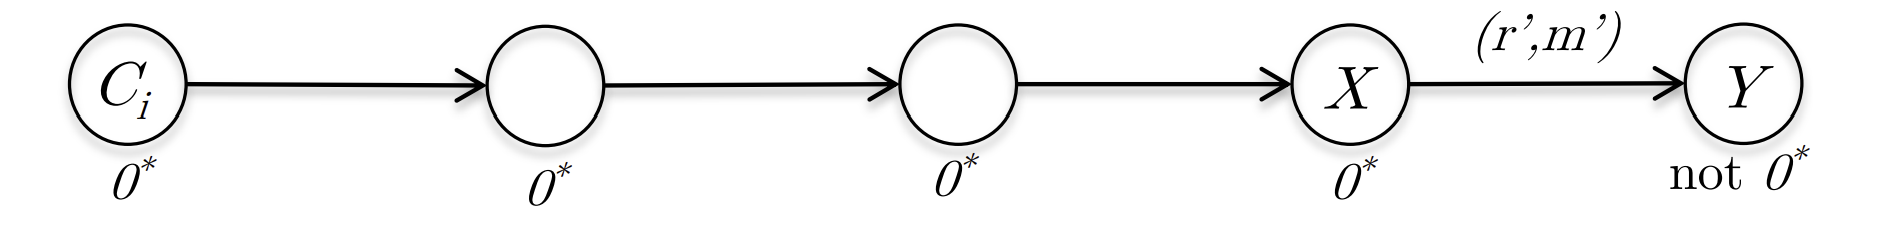
\includegraphics[scale = 0.5]{figures/f18.png}
    \caption{Let $Y$ denote the non-$0^*$-configuration that can be reached from $C_i$ via the delivery of the fewest number of messages (none of which are $(r, m)$), and $X$ its predecessor
configuration on this shortest path.}
    \label{fig:mesh1}
\end{figure}\\
\begin{figure}[h]
    \centering
    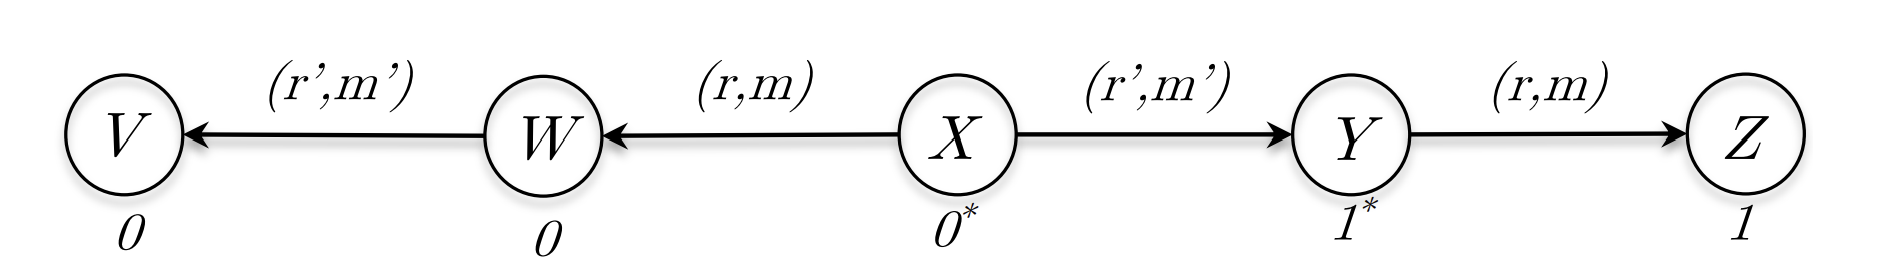
\includegraphics[scale = 0.5]{figures/f19.png}
    \caption{ If $Y$ is a $1^*$-configuration, the order of the delivery of the messages $(r, m)$
and $(r', m')$ starting from configuration $X$ dictates whether the protocol halts with the
all-zero or the all-one outcome.}
    \label{fig:mesh1}
\end{figure}\\

\noindent
\textbf{A pivotal pair of messages.} The key takeaway from Figure 5.4 is that, starting from the
configuration X (whose message pool contains both $(r, m)$ and $(r', m')$):\\
\noindent
(P1) Delivering message $(r, m)$ followed by $(r', m')$ results in a 0-configuration (namely, $V$).\\
\noindent
(P2) Delivering message $(r', m')$ followed by $(r, m)$ results in a 1-configuration (namely, $Z$).\\

In other words, starting from the configuration $X$, the relative order in which the messages $(r, m)$ and $(r', m')$ are received by their recipients is pivotal information and completely
dictates whether the protocol’s final outcome is the all-zero or the all-one outcome (flip their
order and you’ll flip the outcome). Perhaps you can sense the looming contradiction? We’ll
prove it using two cases—the first one direct and easy (and with no Byzantine nodes needed),
the second one similar to our argument in the proof of Lemma 4.6.1.\\

\noindent
\textbf{Case 1:} $r \neq r'$. If the two messages in question are bound to different recipients, then
no node is aware of the relative order in which they were received. (Remember: all a node
knows is its private input and the sequence of messages it has received itself, and its behavior
is completely determined by this knowledge. It does not directly know anything about the
sequences of messages received by other nodes.) Flipping the order in which the messages
are received does not affect the sequence of messages received at any node (or any private
inputs), so all nodes operate identically either way (and in particular, output the same thing).
This contradicts statements (P1) and (P2).\\

\noindent
\textbf{Case 2:} $r = r'$. If the two messages are bound to the same recipient $r$, then node $r$ and
node $r$ alone knows the relative order in which the messages were delivered. (The analog in
the proof of Lemma 4.6.1 is the alleged node with the pivotal private input.) But if $r$ happens
to be the Byzantine node, it is fully capable of hiding from the other nodes the true order in
which it received $(r, m)$ and $(r', m')$, keeping them in the dark. To make that idea precise,
suppose node $r$ is Byzantine and consider two possible strategies for it:
\begin{enumerate}[label=(\roman*)]
    \item follow the protocol $\pi$ honestlym
    \item pretend that it received the messages $(r, m)$ and otherwise follow $\pi$ honestly.
\end{enumerate}
Nodes other than $r$ cannot distinguish between and therefore operate identically in two
scenarios: node $r$ received message $(r, m)$ before $(r', m')$ and is acting honestly (strategy (i)),
node $r$ received $(r',m')$ before $(r, m)$ and is using strategy (ii). This contradicts the facts
that the all-zero outcome is forced in the first scenario (by (P1)) and the all-one outcome
if forced in the second scenario (by (P2)). This contradiction implies the incorrectness of
our assumption that the configuration $Y$ was not an $\text{ambiguous}^*$
configuration. Hence, $Y$ is exactly the type of configuration we were hunting for.

\section{Discussion}
Congratulations! You've survived the not-at-all easy proof of the famous FLP impossibility
theorem, which puts you in the rarified company of distributed computing experts. Before
moving on to climb further mountaintops in the next chapter, let’s not forget the forest for
the trees.\\
First, remember that the point of impossibility results is not to discourage anybody from
trying to come up with really cool consensus or blockchain protocols. Rather, the point is
to educate everybody about the design choices that must be made, the compromises that
must be accepted. For example, the FLP impossibility result (and its extension to the SMR
problem) specifically teaches you that every blockchain consensus protocol
must choose between consistency (all nodes stay in sync) and liveness (transactions keep
getting processed) when the network is under attack. This choice is a top-level node in the
decision tree of blockchain protocol design, with “BFT-type” protocols (like Tendermint in
Chapter 7) favoring consistency when under attack and longest-chain protocols (introduced
in Chapter 8) favoring liveness. No matter how smart you are, you’ll never come up with a
protocol that guarantees the best of both worlds.\\
Second, impossibility results clarify which assumptions matter. For example, Chapter 2
and 3 showed that the PKI assumption (and the existence of cryptography) really matters
(at least in the synchronous model), with results achievable under this trusted setup assumption that are provably impossible without it. Similarly, the FLP impossibility result confirms and formalizes the intuition that the synchrony assumption of Chapter 2 and 3
really matters—the degree of network reliability fundamentally changes what consensus protocols can accomplish.
Third, impossibility results guide you toward the minimal assumptions necessary for
the existence of protocols with provable guarantees. Next chapter, Chapter 6, discusses the
partially synchronous model, which was explicitly conceived as a compromise between the
unrealistic synchronous model and the overly demanding asynchronous model. It’s not clear
anyone would have come up with that “sweet spot” model—arguably the most important one
for assessing the basic properties of blockchain consensus protocols—without the guidance
provided by the FLP impossibility result.\\
Finally, speaking as a theoretician, how cool are these proofs? The impossibility results
from the past few chapters are among the greatest hits of computer science. And even
though our eyes are focused primarily on the future in this chapter series, it’s also important
to celebrate the past—especially when the past remains so practically relevant. Just as many
find it spiritually nourishing to experience fine works of art, perhaps at least a subset of you
will have a similar feeling when internalizing these proofs by the brilliant computer scientists
who have preceded us.















